\documentclass[t]{beamer}
\usetheme{Copenhagen}
\usepackage{amsmath, tikz, bm, pgfplots}
\pgfplotsset{compat=newest}
\pgfplotsset{every tick label/.append style={font=\scriptsize}}
\setbeamertemplate{headline}{} % remove toc from headers
\beamertemplatenavigationsymbolsempty
\everymath{\displaystyle}
% \usepackage[utf8]{inputenc}

\title{Finding Limits: Numerically and Graphically}
\author{}
\date{}

\AtBeginSection[]
{
  \begin{frame}
    \frametitle{Objectives}
    \tableofcontents[currentsection]
  \end{frame}
}

\begin{document}

\begin{frame}{}
    \maketitle
\end{frame}

\section{Understand Limit Notation}

\begin{frame}{Intro}
As we increase the term numbers of a sequence such as
    \[
    1, \frac{1}{2}, \frac{1}{4}, \frac{1}{8}, \dots
    \]
    notice how the values of the terms get closer and closer to 0.   \newline\\  \pause
    
It \alert{may or may not equal 0} at some point, but we would say {\color{blue}\textbf{the limit of the sequence is 0.}}
\end{frame}

\begin{frame}{Limit Notation}
Like sequences, functions can also have limits. \newline\\  \pause
    
To indicate the limit $L$ of a function $f(x)$ as $x$ approaches the value of $a$, we use the notation
\[
\lim_{x \to a} f(x) = L
\]
\pause

This is read    \newline\\
\begin{quote}
    The limit of $f(x)$ as $x$ approaches $a$ is $L$.
\end{quote}
\end{frame}

\begin{frame}{Limit Notation}
    In other words, as $x$ gets closer to the $x$-coordinate $a$, the $y$-values get closer to the $y$-coordinate $L$.   \newline\\        \pause
    
    Sometimes you can just plug the value of $a$ into the function. Other times you can't (e.g. might get division by 0).  
\end{frame}

\begin{frame}{Limit Notation}
\begin{center}
    {\color{red}\Huge{\textbf{*** IMPORTANT ***}}}
\end{center}    

Limits only look at what happens {\color{blue}\textbf{as you get closer to the value of $\bm{a}$}}   \newline\\

They \alert{are not concerned with} what the value of the function is \emph{at} that value of $a$.
\end{frame}

\section{Find a a Limit Using a Table}

\begin{frame}{Example 1}
    For $f(x) = \frac{x^2-6x-7}{x-7}$, find $\lim_{x \to 7}f(x)$.    \newline\\ \pause

$f(7)$ will give us an error message, but what happens if we plug in values of $x$ that are \emph{really close} to 7?    \newline\\  \pause

\begin{minipage}{0.4\textwidth}
\begin{tabular}{cc}
    $\bm{x}$ & $\bm{f(x)}$ \\ \hline  
    \onslide<3->{6.99 & 7.99} \\
    \onslide<4->{6.999 & 7.999 }\\
    \onslide<5->{6.9999 & 7.9999} \\
    \onslide<6->{$\downarrow$ & $\downarrow$} \\
    \onslide<7->{7 & {} }\\
    \onslide<10->{$\uparrow$ & $\uparrow$} \\
    \onslide<10->{7.0001 & 8.0001} \\
    \onslide<9->{7.001 & 8.001} \\
    \onslide<8->{7.01 & 8.01} \\
\end{tabular}
\end{minipage}
\hspace{0.5cm}
\begin{minipage}{0.4\textwidth}
\onslide<11->{$\lim_{x \to 7} f(x) = 8$}
\end{minipage}
\end{frame}

\begin{frame}{Example 2}
    For $f(x) = 3x + 5$, find $\lim_{x \to 2} f(x)$
\newline\\
\begin{minipage}{0.4\textwidth}
\begin{tabular}{cc}
    $\bm{x}$ & $\bm{f(x)}$ \\ \hline  
    \onslide<2->{1.99 & 10.97} \\
    \onslide<3->{1.999 & 10.997 }\\
    \onslide<4->{1.9999 & 10.9997} \\
    \onslide<5->{$\downarrow$ & $\downarrow$} \\
    \onslide<5->{2 & {} }\\
    \onslide<9->{$\uparrow$ & $\uparrow$} \\
    \onslide<8->{2.0001 & 11.0003} \\
    \onslide<7->{2.001 & 11.003} \\
    \onslide<6->{2.01 & 11.03} \\
\end{tabular}
\end{minipage}
\hspace{0.5cm}
\begin{minipage}{0.4\textwidth}
\onslide<10->{$\lim_{x \to 2} f(x) = 11$}
\end{minipage}
\end{frame}

\begin{frame}{Example 3}
    Find $\lim_{x \to 5} \left(\frac{x^3-125}{x-5}\right)$  \newline\\
\begin{minipage}{0.4\textwidth}
\begin{tabular}{cc}
    $\bm{x}$ & $\bm{f(x)}$ \\ \hline  
    \onslide<3->{4.99 & 74.8501} \\
    \onslide<4->{4.999 & 74.985001 }\\
    \onslide<5->{4.9999 & 74.9985} \\
    \onslide<6->{$\downarrow$ & $\downarrow$} \\
    \onslide<7->{5 & {} }\\
    \onslide<10->{$\uparrow$ & $\uparrow$} \\
    \onslide<10->{5.00000001 & 75.000001} \\
    \onslide<9->{5.000001 & 75.000015} \\
    \onslide<8->{5.001 & 75.0015} \\
\end{tabular}
\end{minipage}
\hspace{0.5cm}
\begin{minipage}{0.4\textwidth}
\onslide<11->{$\lim_{x \to 5} \frac{x^3-125}{x-5} = 75$}
\end{minipage}
\end{frame}

\begin{frame}{Example 4}
    Find the limit. \emph{Note:} $x$ is in \underline{radians}.
    \[
    \lim_{x \to 0} \frac{\sin x}{x}
    \]
\begin{minipage}{0.4\textwidth}
\begin{tabular}{cc}
    $\bm{x}$ & $\bm{f(x)}$ \\ \hline  
    \onslide<3->{$-0.001$ & 0.99999983} \\
    \onslide<4->{$-0.0001$ & 1 }\\
    \onslide<5->{$-0.00000001$ & 1} \\
    \onslide<6->{$\downarrow$ & $\downarrow$} \\
    \onslide<7->{0 & {} }\\
    \onslide<10->{$\uparrow$ & $\uparrow$} \\
    \onslide<10->{0.000000001 & 1} \\
    \onslide<9->{0.00001 & 1} \\
    \onslide<8->{0.001 & 0.99999983} \\
\end{tabular}
\end{minipage}
\hspace{0.5cm}
\begin{minipage}{0.4\textwidth}
\onslide<11->{$\lim_{x \to 0} \frac{\sin x}{x} = 1$}
\end{minipage}
\end{frame}

\begin{frame}{Left-Hand and Right-Hand Limits}
    In the previous examples, we found limits by evaluating values less than the value of $a$ and also values greater than $a$. \newline\\
    
    These are called \alert{left-hand limits} and \alert{right-hand limits}, respectively.
\end{frame}

\begin{frame}{Left-Hand Limit}
    \[
    f(x) = \frac{x^2-6x-7}{x-7}
    \]
    \newline\\
    \begin{center}
    \begin{tabular}{c|c|c|c|c|}
        {} & \multicolumn{3}{|c|}{Values of $x$ approach 7 from the left ($x < 7$)} & \\ \hline
        $x$ & 6.99 & 6.999 & 6.9999 & 7 \\[6pt]
        $f(x)$ & \alert{7.99} & \alert{7.999} & \alert{7.9999} & Undefined \\[8pt]
    \end{tabular}
        \end{center}
    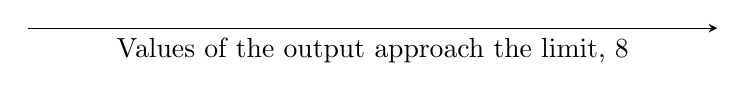
\begin{tikzpicture}
    \draw[->, >=stealth] (0,0) -- (8.75,0) node [below, midway] {Values of the output approach the limit, \alert{8}};
    \end{tikzpicture}
\end{frame}

\begin{frame}{Right-Hand Limit}
    \[
    f(x) = \frac{x^2-6x-7}{x-7}
    \]
    \newline\\
    \begin{center}
    \begin{tabular}{c|c|c|c|c|}
        {} & & \multicolumn{3}{|c|}{Values of $x$ approach 7 from the right ($x < 7$)} \\ \hline
        $x$ & 7 & 7.0001 & 7.001 & 7.01 \\[6pt]
        $f(x)$ & Undefined & \alert{8.001} & \alert{8.01} & \alert{8.01} \\[8pt]
    \end{tabular}
        \end{center}
    \begin{flushright}
    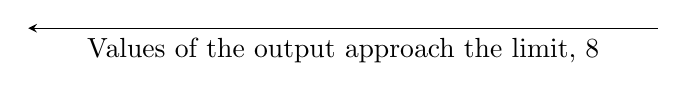
\begin{tikzpicture}
    \draw[<-, >=stealth] (4.5,0) -- (12.5,0) node [midway, below] {Values of the output approach the limit, \alert{8}};
    \end{tikzpicture}
    \end{flushright}
\end{frame}

\begin{frame}[c]{Notation}
\begin{center}
    \begin{tabular}{p{0.3\textwidth}c}
        Left-Hand Limit: & $\lim_{x\to a^-} f(x)$ \\[18pt]
        \onslide<2->{Right-Hand Limit: & $\lim_{x\to a^+} f(x)$} \\
    \end{tabular}
\end{center}
\end{frame}

\begin{frame}[c]{Two-Sided Limit}
    \begin{center}
    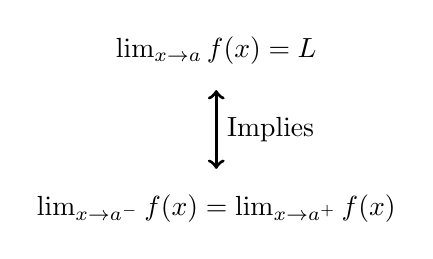
\begin{tikzpicture}
    \node at (0,0) {$\lim_{x \to a} f(x) = L$};
    \draw [<->, very thick] (0,-0.5) -- (0,-1.5) node [midway, right] {Implies};
    \node at (0,-2) {$\lim_{x \to a^-} f(x) = \lim_{x\to a^+} f(x)$};
    \end{tikzpicture}
    \end{center}
\end{frame}


\section{Find a Limit Using a Graph}

\begin{frame}{Finding a limit using a graph}
    For $f(x)$ as $x$ approaches $a$:   \newline\\  \pause
    \begin{itemize}
        \item Examine the graph to see if left-hand limit exists.\newline\\  \pause
        \begin{itemize}
            \item Won't if there is a vertical asymptote at $x=a$\newline\\  \pause
        \end{itemize}
        \item Examine the graph to see if right-hand limit exists.\newline\\  \pause
        \begin{itemize}
            \item Ditto from above\newline\\  \pause
        \end{itemize}
        \item If the 2 one-sided limits exist and are equal, there is a ``limit."\newline\\  \pause
        \item If there is a point at $x = a$, then $f(a)$ is the value of the function at $x=a$.
    \end{itemize}
\end{frame}

\begin{frame}{Example 5}
    Use the graph of $f(x)$ to find each.   \newline\\
\begin{minipage}{0.6\textwidth}
    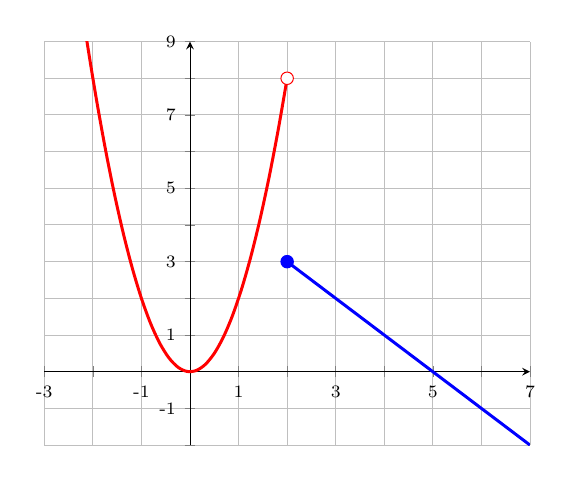
\begin{tikzpicture}[scale=0.9]
    \begin{axis}[
    xmin = -3, xmax =7,
    ymin = -2, ymax = 9,
    axis lines = middle,
    grid,
    xtick = {-3,-2,...,7},
    ytick = {-2,-1,...,9},
    xticklabels = {-3,,-1,,1,,3,,5,,7},
    yticklabels = {,-1,,1,,3,,5,,7,,9}
    ]
    \addplot[color=red,domain=-2.5:2,smooth,very thick] {2*x^2};
    \addplot[color=blue,domain=2:7,smooth,very thick] {5-x};
    \addplot[mark = *, mark size = 2.5pt, color=blue] coordinates {(2,3)};
    \addplot[mark = *, mark size = 2.5pt, color=red, fill=white] coordinates {(2,8)};
    \end{axis}
    \end{tikzpicture}
\end{minipage}
\hspace{-0.25cm}
\begin{minipage}{0.4\textwidth}
    \begin{align*}
    (a)& \quad \lim_{x\to 2^-} f(x) \onslide<2->{= {\color{red}8}} \\[10pt]
    \onslide<3->{(b)& \quad \lim_{x\to 2^+} f(x) } 
    \onslide<4->{= {\color{blue}3}} \\[10pt]
    \onslide<5->{(c)& \quad \lim_{x\to 2} f(x) }
    \onslide<6->{=\text{DNE}} \\[10pt]
    \onslide<7->{(d)& \quad f(2) }
    \onslide<8->{= 3} \\
    \end{align*}
\end{minipage}
\end{frame}

\begin{frame}{Example 6}
Use the graph of $f(x)$ to find each.   \newline\\
\begin{minipage}{0.6\textwidth}
    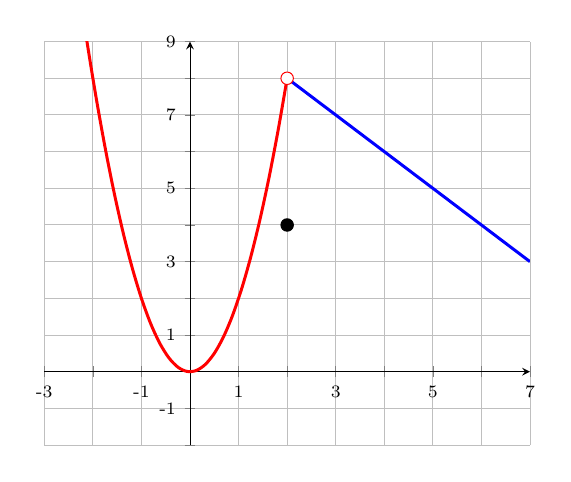
\begin{tikzpicture}[scale=0.9]
    \begin{axis}[
    xmin = -3, xmax =7,
    ymin = -2, ymax = 9,
    axis lines = middle,
    grid,
    xtick = {-3,-2,...,7},
    ytick = {-2,-1,...,9},
    xticklabels = {-3,,-1,,1,,3,,5,,7},
    yticklabels = {,-1,,1,,3,,5,,7,,9}
    ]
    \addplot[color=red,domain=-2.5:2,smooth,very thick] {2*x^2};
    \addplot[color=blue,domain=2:7,smooth,very thick] {10-x};
    \addplot[mark = *, mark size = 2.5pt] coordinates {(2,4)};
    \addplot[mark = *, mark size = 2.5pt, color=red, fill=white] coordinates {(2,8)};
    \end{axis}
    \end{tikzpicture}
\end{minipage}
\hspace{-0.25cm}
\begin{minipage}{0.4\textwidth}
    \begin{align*}
    (a)& \quad \lim_{x\to 2^-} f(x) \onslide<2->{= {\color{red}8}} \\[10pt]
    \onslide<3->{(b)& \quad \lim_{x\to 2^+} f(x) } 
    \onslide<4->{= {\color{blue}8}} \\[10pt]
    \onslide<5->{(c)& \quad \lim_{x\to 2} f(x) }
    \onslide<6->{= {\color{violet}8}} \\[10pt]
    \onslide<7->{(d)& \quad f(2) }
    \onslide<8->{= 4} \\
    \end{align*}
\end{minipage}    
\end{frame}
\end{document}
